\documentclass{article}
\usepackage{amsmath}
\usepackage{multicol}
\usepackage[paperwidth=5.5in, paperheight=8.5in, margin=0.2in]{geometry}
\usepackage{pgfplots}
\pgfplotsset{compat=1.18}
\usepackage{graphicx} % Required for inserting images
\usepackage{tgadventor}
\renewcommand*\familydefault{\sfdefault} %% Only if the base font of the document is to be sans serif
\usepackage[T1]{fontenc}

\pgfplotsset{
    every axis/.append style={
        scale only axis,
        width=0.75\textwidth,
        xtick={0,0.05,0.1},
    }
}
\begin{document}
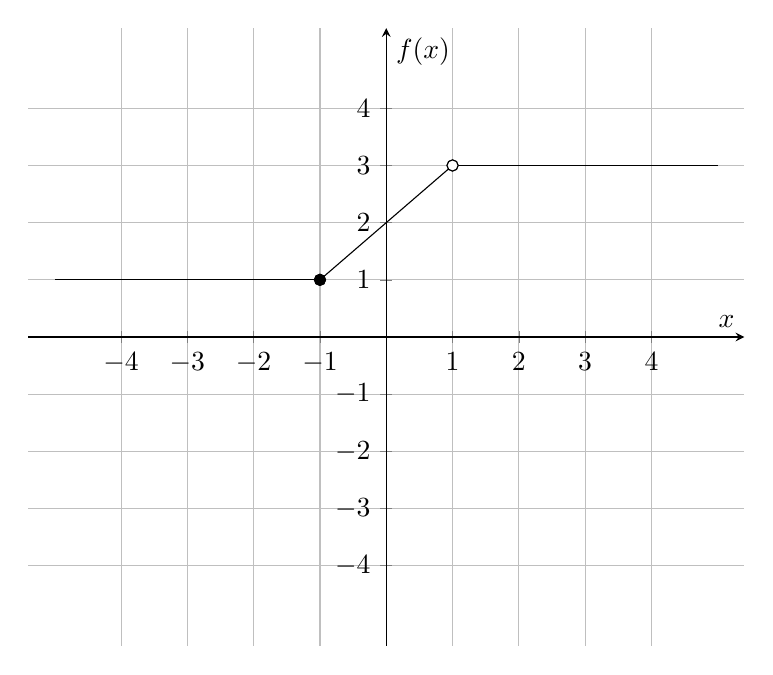
\begin{tikzpicture}
\begin{axis}[axis lines = middle,
            xlabel = $x$, ylabel = $f(x)$,
            domain=-4:4,
            samples=20,
            ymin=-4.5, ymax=4.5,
            xmin=-4.5, xmax=4.5,
            grid=both,
            xtick={-4,-3,-2,-1,1,2,3,4},
            ytick={-4,-3,-2,-1,1,2,3,4},
            enlargelimits=true]

\addplot[domain=-5:-1]{1*x^0};
\addplot[domain=-1:1]{1*x^1+2*x^0};
\addplot[domain=1:5]{3*x^0};
% Open circles at discontinuities
\addplot[only marks, mark=*, fill=white] coordinates{(-inf,1.0)};
\addplot[only marks, mark=*, fill=white] coordinates{(-1,1)};
\addplot[only marks, mark=*, fill=black] coordinates{(-1,1)};
\addplot[only marks, mark=*, fill=black] coordinates{(1,3)};
\addplot[only marks, mark=*, fill=white] coordinates{(1,3)};
\addplot[only marks, mark=*, fill=white] coordinates{(inf,3.0)};
\end{axis}
\end{tikzpicture}

brash
\vspace{2in}
\hrule
\vspace{0.5in}

graph holds constant at 1 until x=-1, then rises until it hits 3 at x=1, then stays constant at 3

\vspace{2ex}
Liam

\pagebreak
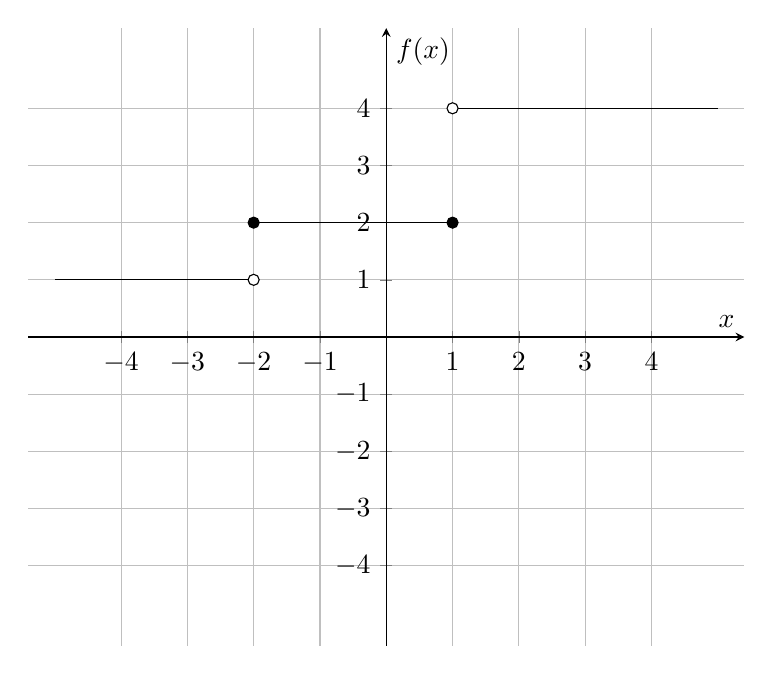
\begin{tikzpicture}
\begin{axis}[axis lines = middle,
            xlabel = $x$, ylabel = $f(x)$,
            domain=-4:4,
            samples=20,
            ymin=-4.5, ymax=4.5,
            xmin=-4.5, xmax=4.5,
            grid=both,
            xtick={-4,-3,-2,-1,1,2,3,4},
            ytick={-4,-3,-2,-1,1,2,3,4},
            enlargelimits=true]

\addplot[domain=-5:-2]{1*x^0};
\addplot[domain=-2:1]{2*x^0};
\addplot[domain=1:5]{4*x^0};
% Open circles at discontinuities
\addplot[only marks, mark=*, fill=white] coordinates{(-inf,1.0)};
\addplot[only marks, mark=*, fill=white] coordinates{(-2,1)};
\addplot[only marks, mark=*, fill=black] coordinates{(-2,2)};
\addplot[only marks, mark=*, fill=black] coordinates{(1,2)};
\addplot[only marks, mark=*, fill=white] coordinates{(1,4)};
\addplot[only marks, mark=*, fill=white] coordinates{(inf,4.0)};
\end{axis}
\end{tikzpicture}

bumpy
\vspace{2in}
\hrule
\vspace{0.5in}

graph is constant at a value of 1 until x=-2, where it jumps up by one, and holds constant, then jumps up by two at x=1, and is constant forever after.

\vspace{2ex}
Ava

\pagebreak
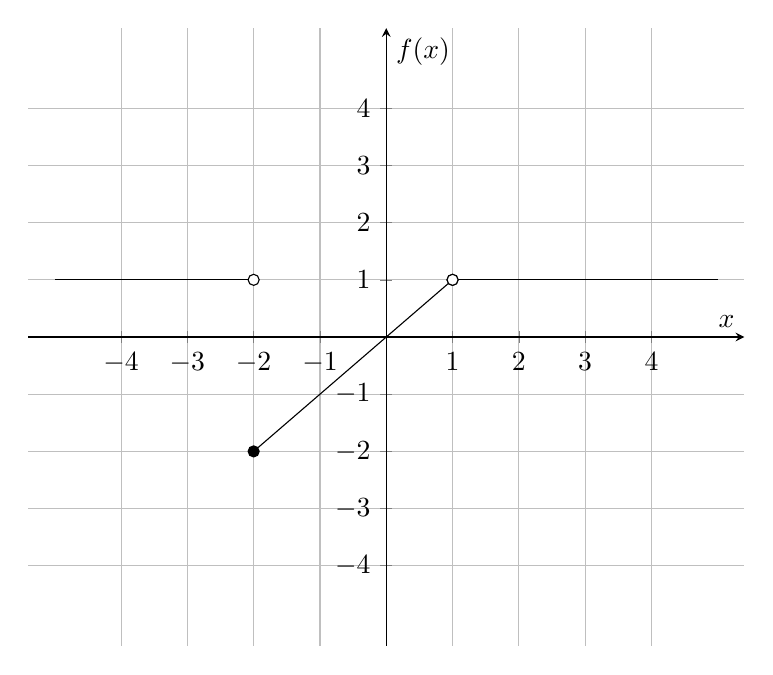
\begin{tikzpicture}
\begin{axis}[axis lines = middle,
            xlabel = $x$, ylabel = $f(x)$,
            domain=-4:4,
            samples=20,
            ymin=-4.5, ymax=4.5,
            xmin=-4.5, xmax=4.5,
            grid=both,
            xtick={-4,-3,-2,-1,1,2,3,4},
            ytick={-4,-3,-2,-1,1,2,3,4},
            enlargelimits=true]

\addplot[domain=-5:-2]{1*x^0};
\addplot[domain=-2:1]{1*x^1};
\addplot[domain=1:5]{1*x^0};
% Open circles at discontinuities
\addplot[only marks, mark=*, fill=white] coordinates{(-inf,1.0)};
\addplot[only marks, mark=*, fill=white] coordinates{(-2,1)};
\addplot[only marks, mark=*, fill=black] coordinates{(-2,-2)};
\addplot[only marks, mark=*, fill=black] coordinates{(1,1)};
\addplot[only marks, mark=*, fill=white] coordinates{(1,1)};
\addplot[only marks, mark=*, fill=white] coordinates{(inf,1.0)};
\end{axis}
\end{tikzpicture}

clumsy
\vspace{2in}
\hrule
\vspace{0.5in}

\begin{tabular}{|c|c|}
\hline
$x$ & $f(x)$ \\
\hline
-4 & 1 \\
\hline
-3 & 1 \\
\hline
-2 & -2 \\
\hline
-1 & -1 \\
\hline
0 & 0 \\
\hline
1 & 1 \\
\hline
2 & 1 \\
\hline
3 & 1 \\
\hline
\end{tabular}


\vspace{2ex}
Soraya

\pagebreak
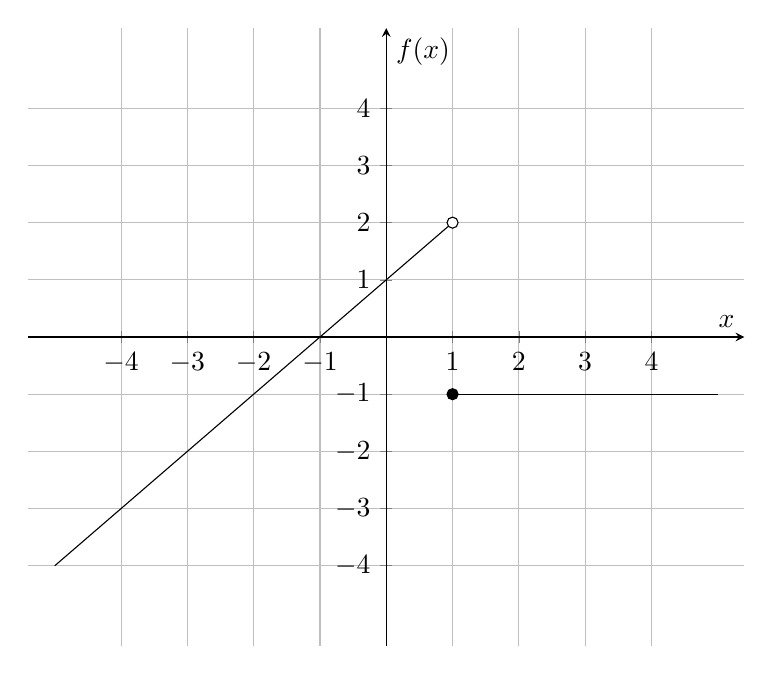
\begin{tikzpicture}
\begin{axis}[axis lines = middle,
            xlabel = $x$, ylabel = $f(x)$,
            domain=-4:4,
            samples=20,
            ymin=-4.5, ymax=4.5,
            xmin=-4.5, xmax=4.5,
            grid=both,
            xtick={-4,-3,-2,-1,1,2,3,4},
            ytick={-4,-3,-2,-1,1,2,3,4},
            enlargelimits=true]

\addplot[domain=-5:1]{1*x^1+1*x^0};
\addplot[domain=1:5]{-1*x^0};
% Open circles at discontinuities
\addplot[only marks, mark=*, fill=white] coordinates{(-inf,-inf)};
\addplot[only marks, mark=*, fill=white] coordinates{(1,2)};
\addplot[only marks, mark=*, fill=black] coordinates{(1,-1)};
\addplot[only marks, mark=*, fill=white] coordinates{(inf,-1.0)};
\end{axis}
\end{tikzpicture}

dazzling
\vspace{2in}
\hrule
\vspace{0.5in}

\begin{tabular}{|c|c|}
\hline
$x$ & $f(x)$ \\
\hline
-4 & -3 \\
\hline
-3 & -2 \\
\hline
-2 & -1 \\
\hline
-1 & 0 \\
\hline
0 & 1 \\
\hline
1 & -1 \\
\hline
2 & -1 \\
\hline
3 & -1 \\
\hline
\end{tabular}


\vspace{2ex}
Ronan

\pagebreak
\begin{align*}
f(x)=
\begin{cases}
x +1 & \text{ if } x < 1 \\ 
1 & \text{ if } x \geq 1
\end{cases}
\end{align*}

eerie
\vspace{2in}
\hrule
\vspace{0.5in}

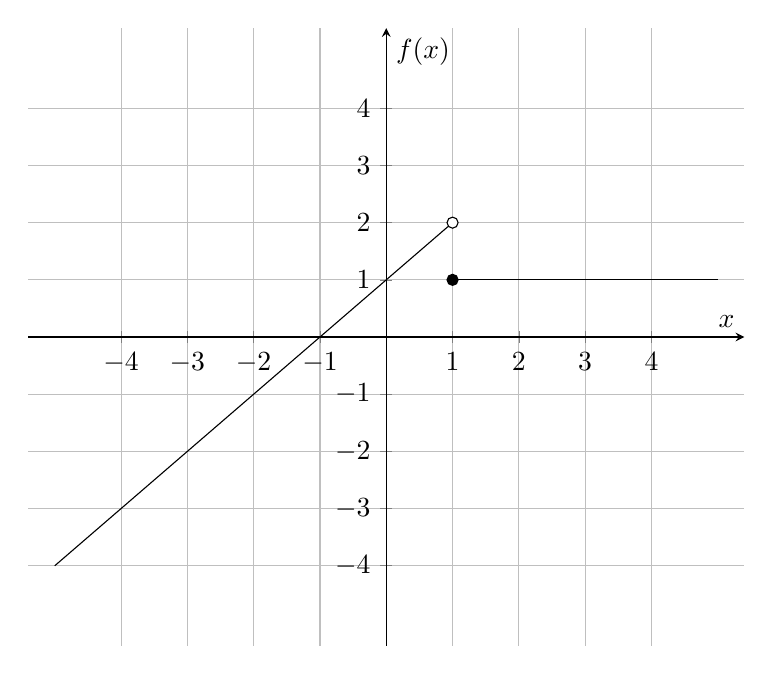
\begin{tikzpicture}
\begin{axis}[axis lines = middle,
            xlabel = $x$, ylabel = $f(x)$,
            domain=-4:4,
            samples=20,
            ymin=-4.5, ymax=4.5,
            xmin=-4.5, xmax=4.5,
            grid=both,
            xtick={-4,-3,-2,-1,1,2,3,4},
            ytick={-4,-3,-2,-1,1,2,3,4},
            enlargelimits=true]

\addplot[domain=-5:1]{1*x^1+1*x^0};
\addplot[domain=1:5]{1*x^0};
% Open circles at discontinuities
\addplot[only marks, mark=*, fill=white] coordinates{(-inf,-inf)};
\addplot[only marks, mark=*, fill=white] coordinates{(1,2)};
\addplot[only marks, mark=*, fill=black] coordinates{(1,1)};
\addplot[only marks, mark=*, fill=white] coordinates{(inf,1.0)};
\end{axis}
\end{tikzpicture}


\vspace{2ex}
Hadley

\pagebreak
\begin{align*}
f(x)=
\begin{cases}
1 & \text{ if } x < -2 \\ 
-x & \text{ if } -2 \leq x \leq 1 \\ 
1 & \text{ if } x > 1
\end{cases}
\end{align*}

fierce
\vspace{2in}
\hrule
\vspace{0.5in}

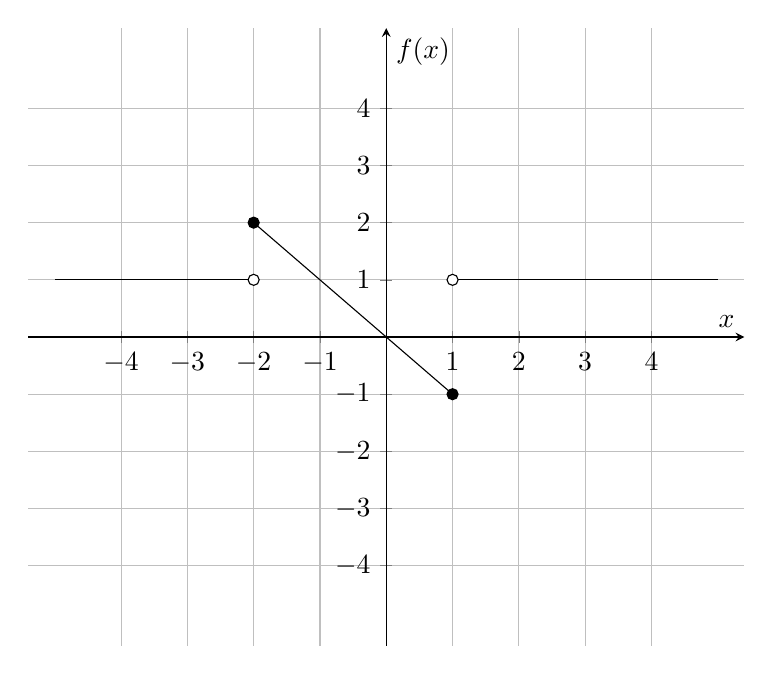
\begin{tikzpicture}
\begin{axis}[axis lines = middle,
            xlabel = $x$, ylabel = $f(x)$,
            domain=-4:4,
            samples=20,
            ymin=-4.5, ymax=4.5,
            xmin=-4.5, xmax=4.5,
            grid=both,
            xtick={-4,-3,-2,-1,1,2,3,4},
            ytick={-4,-3,-2,-1,1,2,3,4},
            enlargelimits=true]

\addplot[domain=-5:-2]{1*x^0};
\addplot[domain=-2:1]{-1*x^1};
\addplot[domain=1:5]{1*x^0};
% Open circles at discontinuities
\addplot[only marks, mark=*, fill=white] coordinates{(-inf,1.0)};
\addplot[only marks, mark=*, fill=white] coordinates{(-2,1)};
\addplot[only marks, mark=*, fill=black] coordinates{(-2,2)};
\addplot[only marks, mark=*, fill=black] coordinates{(1,-1)};
\addplot[only marks, mark=*, fill=white] coordinates{(1,1)};
\addplot[only marks, mark=*, fill=white] coordinates{(inf,1.0)};
\end{axis}
\end{tikzpicture}


\vspace{2ex}
Jack

\pagebreak
\begin{align*}
f(x)=
\begin{cases}
-1 & \text{ if } x < -1 \\ 
x & \text{ if } -1 \leq x \leq 1 \\ 
1 & \text{ if } x > 1
\end{cases}
\end{align*}

foggy
\vspace{2in}
\hrule
\vspace{0.5in}

\begin{tabular}{|c|c|}
\hline
$x$ & $f(x)$ \\
\hline
-4 & -1 \\
\hline
-3 & -1 \\
\hline
-2 & -1 \\
\hline
-1 & -1 \\
\hline
0 & 0 \\
\hline
1 & 1 \\
\hline
2 & 1 \\
\hline
3 & 1 \\
\hline
\end{tabular}


\vspace{2ex}
Elijah

\pagebreak
\begin{align*}
f(x)=
\begin{cases}
-1 & \text{ if } x < -2 \\ 
x & \text{ if } -2 \leq x \leq 2 \\ 
1 & \text{ if } x > 2
\end{cases}
\end{align*}

gaudy
\vspace{2in}
\hrule
\vspace{0.5in}

\begin{tabular}{|c|c|}
\hline
$x$ & $f(x)$ \\
\hline
-4 & -1 \\
\hline
-3 & -1 \\
\hline
-2 & -2 \\
\hline
-1 & -1 \\
\hline
0 & 0 \\
\hline
1 & 1 \\
\hline
2 & 2 \\
\hline
3 & 1 \\
\hline
\end{tabular}


\vspace{2ex}
Sophia

\pagebreak
\begin{center}
\Large Answer Key
\end{center}
\begin{itemize}
\item brash : Liam
\item bumpy : Ava
\item clumsy : Soraya
\item dazzling : Ronan
\item eerie : Hadley
\item fierce : Jack
\item foggy : Elijah
\item gaudy : Sophia
\end{itemize}
\end{document}

